\documentclass[border=10pt]{standalone}
\usepackage[svgnames]{xcolor}
\usepackage{amsmath}
\usepackage{pgfplots}
\pgfplotsset{compat=newest}
\usepackage[sfdefault]{FiraSans}
\usepackage{FiraMono}
\renewcommand*\familydefault{\sfdefault}
\begin{document}
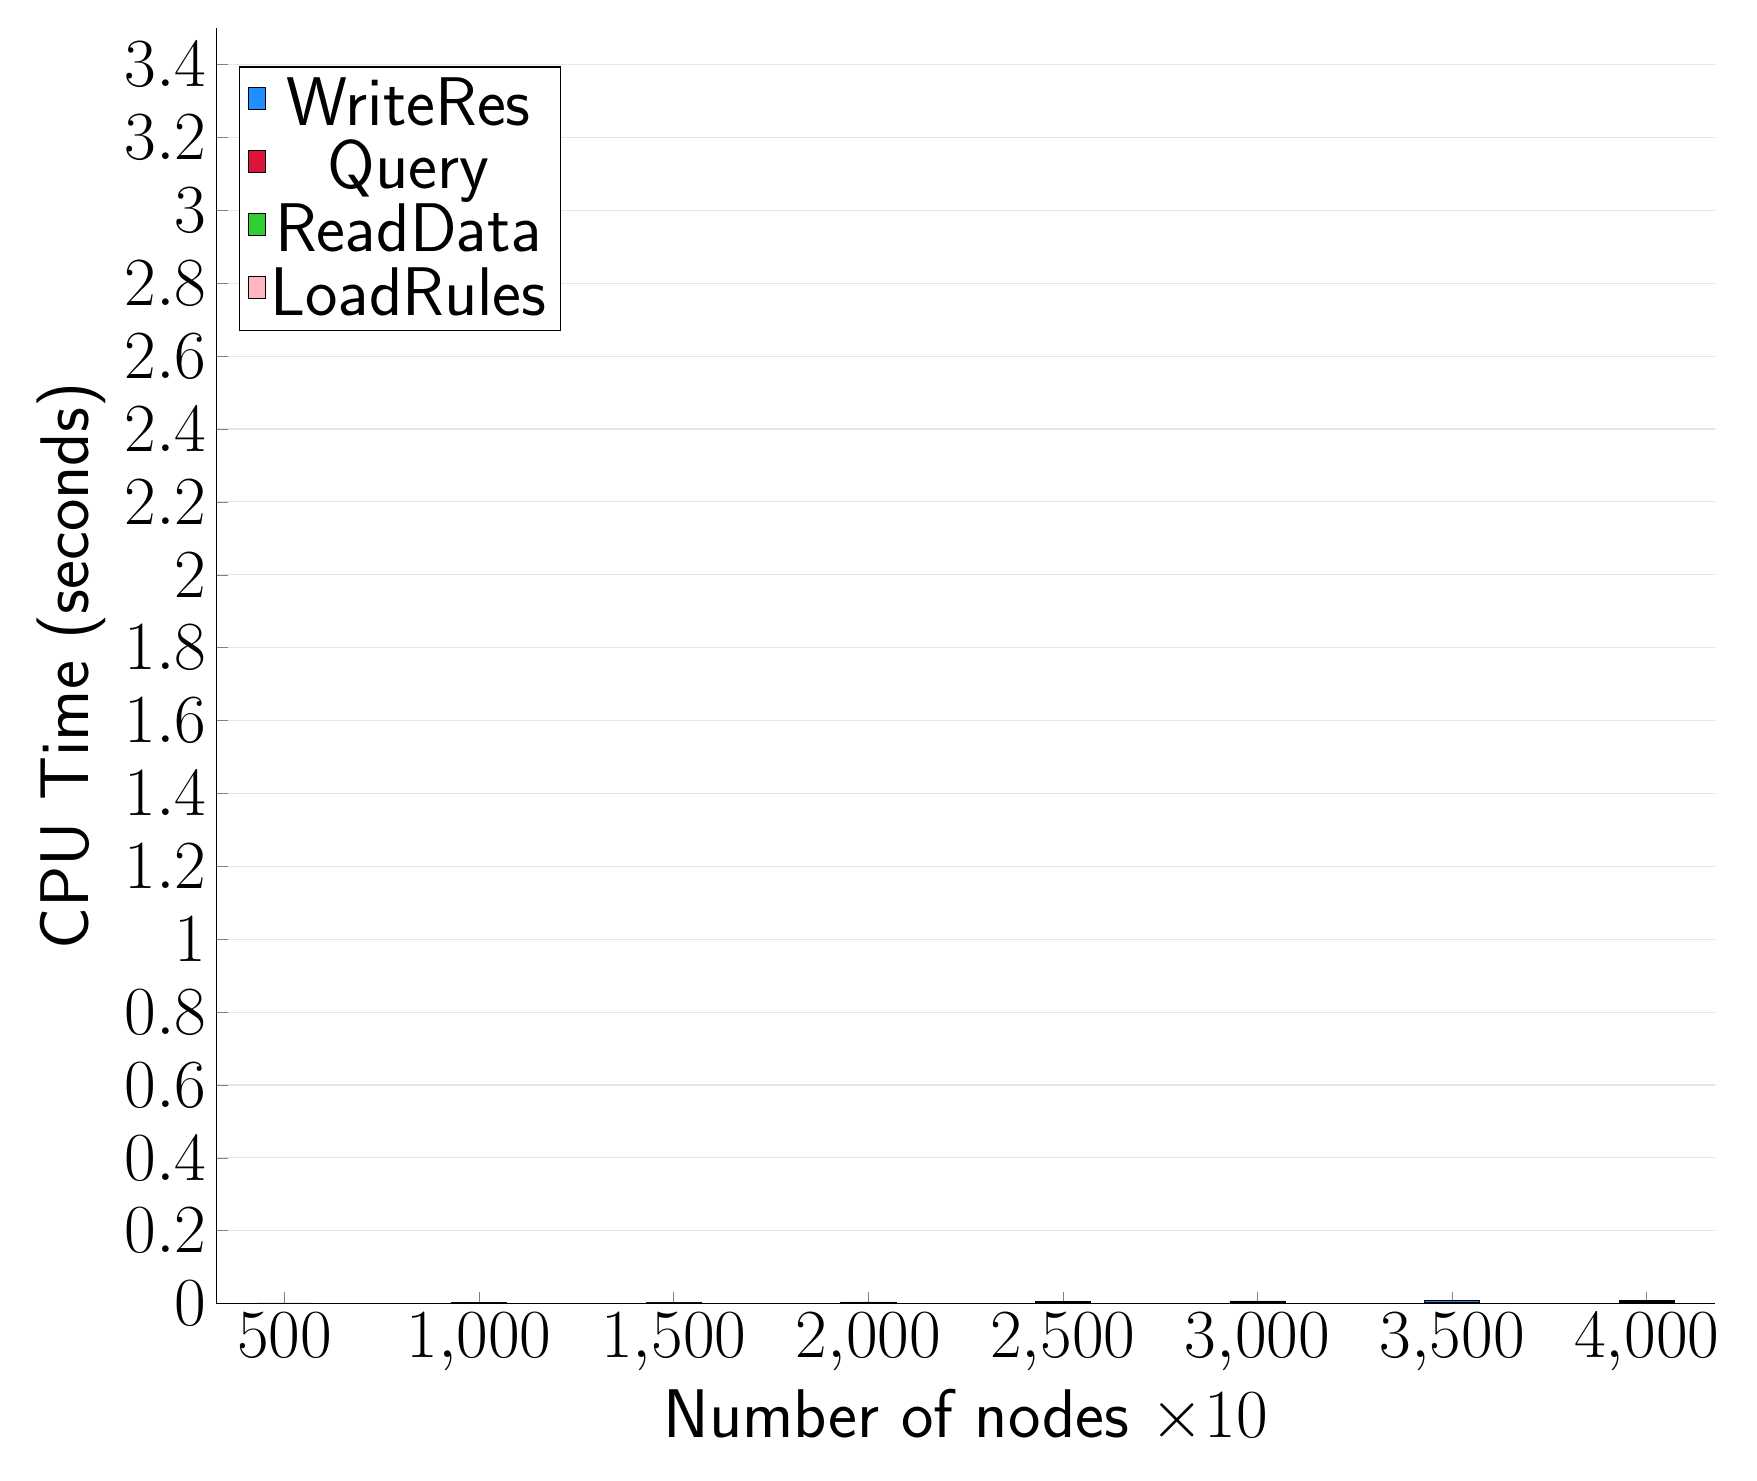
\begin{tikzpicture}
\begin{axis}[
   ybar stacked,
   width=1.7\textwidth,
   bar width=0.7cm,
   ymajorgrids, tick align=inside,
   major grid style={draw=gray!20},
   xtick=data,
   ymin=0, ymax=3.5,
   axis x line*=bottom,
   axis y line*=left,
   enlarge x limits=0.05,
   legend style={
       at={(0.23, 0.97)},
       anchor=north east,
       legend columns=1,
       font=\Huge,
   },
   ylabel={CPU Time (seconds)},
   xlabel={Number of nodes $\times 10$},
   label style={font=\Huge},
   tick label style={font=\Huge},
]
\addlegendimage{fill=DodgerBlue, draw=black, line width=0.2pt}
\addlegendentry{WriteRes}
\addlegendimage{fill=Crimson, draw=black, line width=0.2pt}
\addlegendentry{Query}
\addlegendimage{fill=LimeGreen, draw=black, line width=0.2pt}
\addlegendentry{ReadData}
\addlegendimage{fill=LightPink, draw=black, line width=0.2pt}
\addlegendentry{LoadRules}
\addplot +[fill=LightPink, draw=black, line width=0.2pt] coordinates {
(500, 0.0005996)
(1000, 0.0006213000000000002)
(1500, 0.0006450000000000001)
(2000, 0.0006138999999999998)
(2500, 0.0006094)
(3000, 0.0006635999999999998)
(3500, 0.0006411999999999998)
(4000, 0.0006245000000000003)
};
\addplot +[fill=LimeGreen, draw=black, line width=0.2pt] coordinates {
(500, 0.0005417999999999996)
(1000, 0.0009953000000000004)
(1500, 0.0015178999999999998)
(2000, 0.0019105)
(2500, 0.0023179000000000003)
(3000, 0.0028798)
(3500, 0.0032356999999999998)
(4000, 0.0036857999999999995)
};
\addplot +[fill=Crimson, draw=black, line width=0.2pt] coordinates {
(500, 8.940000000000041e-05)
(1000, 0.0001718999999999993)
(1500, 0.0002629000000000002)
(2000, 0.0003371000000000002)
(2500, 0.0004903000000000002)
(3000, 0.0006750000000000003)
(3500, 0.0008247)
(4000, 0.0009096)
};
\addplot +[fill=DodgerBlue, draw=black, line width=0.2pt] coordinates {
(500, 0.0005165999999999997)
(1000, 0.0009742000000000006)
(1500, 0.0014110999999999996)
(2000, 0.0018723999999999998)
(2500, 0.0023401)
(3000, 0.0030097999999999995)
(3500, 0.0033907)
(4000, 0.003825)
};
\end{axis}
\end{tikzpicture}

\end{document}
